\everymath{\displaystyle}
\documentclass{beamer}
% \documentclass[handout]{beamer}

%\usepackage[pdftex]{color,graphicx}
\usepackage{amsmath,amssymb,amsfonts}

\mode<presentation>
{
  % \usetheme{Darmstadt}
  % \usetheme[hideothersubsections]{Hannover}
  % \usetheme[hideothersubsections]{Goettingen}
  \usetheme[hideothersubsections, right]{Berkeley}

  \usecolortheme{seahorse}
  % \usecolortheme{dolphin}
  \usecolortheme{rose}
  % \usecolortheme{orchid}

  \useinnertheme[shadow]{rounded}

  \setbeamercovered{transparent}
  % or whatever (possibly just delete it)
}

\mode<handout>{
  \setbeamercolor{background canvas}{bg=black!5}
  \usepackage{pgfpages}
  \pgfpagesuselayout{4 on 1}[a4paper,border shrink=5mm, landscape]
}

\usepackage[brazilian]{babel}
% or whatever

% \usepackage[latin1]{inputenc}
\usepackage[utf8]{inputenc}
% or whatever

\usepackage{times}
%\usepackage[T1]{fontenc}
% Or whatever. Note that the encoding and the font should match. If T1
% does not look nice, try deleting the line with the fontenc.


\title%[] % (optional, use only with long paper titles)
{Testes de Hipóteses II}

\subtitle
{O p-valor, e testes com duas amostras} % (optional)

\author%[] % (optional, use only with lots of authors)
{Felipe Figueiredo}% \and S.~Another\inst{2}}
% - Use the \inst{?} command only if the authors have different
%   affiliation.

\institute[INTO] % (optional, but mostly needed)
{Instituto Nacional de Traumatologia e Ortopedia
}
  % \inst{1}%
  % Department of Computer Science\\
  % University of Somewhere
  % \and
  % \inst{2}%
  % Department of Theoretical Philosophy\\
  % University of Elsewhere}
% - Use the \inst command only if there are several affiliations.
% - Keep it simple, no one is interested in your street address.

\date%[] % (optional)
{}

% \subject{Talks}
% This is only inserted into the PDF information catalog. Can be left
% out. 



% If you have a file called "university-logo-filename.xxx", where xxx
% is a graphic format that can be processed by latex or pdflatex,
% resp., then you can add a logo as follows:

\pgfdeclareimage[height=1.6cm]{university-logo}{../logo}
\logo{\pgfuseimage{university-logo}}



% Delete this, if you do not want the table of contents to pop up at
% the beginning of each subsection:
\AtBeginSubsection[]
%\AtBeginSection[]
{
  \begin{frame}<beamer>{Sumário}
    \tableofcontents[currentsection,currentsubsection]
  \end{frame}
}


% If you wish to uncover everything in a step-wise fashion, uncomment
% the following command: 

\beamerdefaultoverlayspecification{<+->}


\begin{document}

\begin{frame}
  \titlepage
\end{frame}

\begin{frame}{Sumário}
  \tableofcontents
  % You might wish to add the option [pausesections]
\end{frame}


%% Template
% \section{}

% \subsection{}

% \begin{frame}{}
%   \begin{itemize}
%   \item 
%   \end{itemize}
% \end{frame}

% \begin{frame}
%   \begin{columns}
%     \begin{column}{5cm}
%     \end{column}
%     \begin{column}{5cm}
%     \end{column}
%   \end{columns}
% \end{frame}

% \begin{frame}{}
%   \includegraphics[height=0.4\textheight]{file1}
%   \includegraphics[height=0.4\textheight]{file2}
%   \includegraphics[height=0.4\textheight]{file3}
%   \begin{figure}
%     \caption{}
%   \end{figure}
% \end{frame}

% \begin{frame}{}
%   \begin{definition}
%   \end{definition}
%   \begin{example}
%   \end{example}
%   \begin{block}{Exercício}
%   \end{block}
% \end{frame}

\section{Testes com uma amostra}

\subsection{Recapitulando}

\begin{frame}{Recapitulando}
  Vimos como formular hipóteses estatísticas seguindo o procedimento
  abaixo:
  \begin{block}{Teste de hipóteses}
    \begin{enumerate}
    \item Formular as hipóteses nula e alternativa
    \item Identificar a região crítica (região de rejeição)
    \item Calcular a estatística de teste adequada
    \item Rejeitar ou não a hipótese nula
    \end{enumerate}
  \end{block}
\end{frame}

\begin{frame}{}
  \begin{itemize}
  \item Este processo sistemático pode ser aplicado a diversos tipos
    de hipóteses em estudos com dados quantitativos.
  \item Atualmente tem se usado com mais frequência uma metodologia
    equivalente usando o \alert{p-valor} (ou valor P).
  \item Diferença: ao invés de comparar diretamente os Z-escores
    (região crítica sob a curva), vamos comparar as probabilidades
    destes (significância)
  \item Envolve premissas sutis e a interpretação deve ser tomada
    cuidadosamente (veja artigos complementares no site).
  \end{itemize}
\end{frame}


\subsection{O p-valor}

\begin{frame}{O p-valor}
  \begin{definition}
    Assumindo que a hipótese nula seja verdadeira, o \alert{p-valor}
    de um teste de hipóteses é a probabilidade de se obter uma
    estatística amostral com valores tão extremos, ou mais extremos
    que aquele observado.
  \end{definition}

O p-valor \alert{é}:
  \begin{itemize}
  \item Uma estatística (i.e., depende da amostra - dados e tamanho)
  \item A probabilidade (condicional) de se observar o resultado ao
    acaso \alert{dado que} a $H_0$ é verdadeira.
  \item Uma medida da força da evidência contra a $H_0$.
  \end{itemize}
\end{frame}

\begin{frame}{O p-valor}
  \begin{block}{Como utilizar}
    \begin{itemize}
    \item Quanto menor o p-valor, mais evidências para rejeitar a
      hipótese nula.
    \item O ponto de corte mais utilizado é a significância de 5\%
    \item Assim, qualquer $p \le 0.05$ é estatisticamente significante.
    \end{itemize}
  \end{block}
\end{frame}

\begin{frame}{O p-valor}
  \begin{block}{Como calcular}
    \begin{itemize}
    \item calcular a estatística de teste apropriada para a situação
      (teste Z, teste t, etc.)
    \item encontrar a probabilidade $p$ correspondente a esta
      estatística (por exemplo, na tabela apropriada, ou com uma
      ferramenta computacional)
    \item comparar o p-valor encontrado com a significância do estudo
    \end{itemize}
  \end{block}
\end{frame}

\begin{frame}{O p-valor}
  \begin{figure}
    \centering
      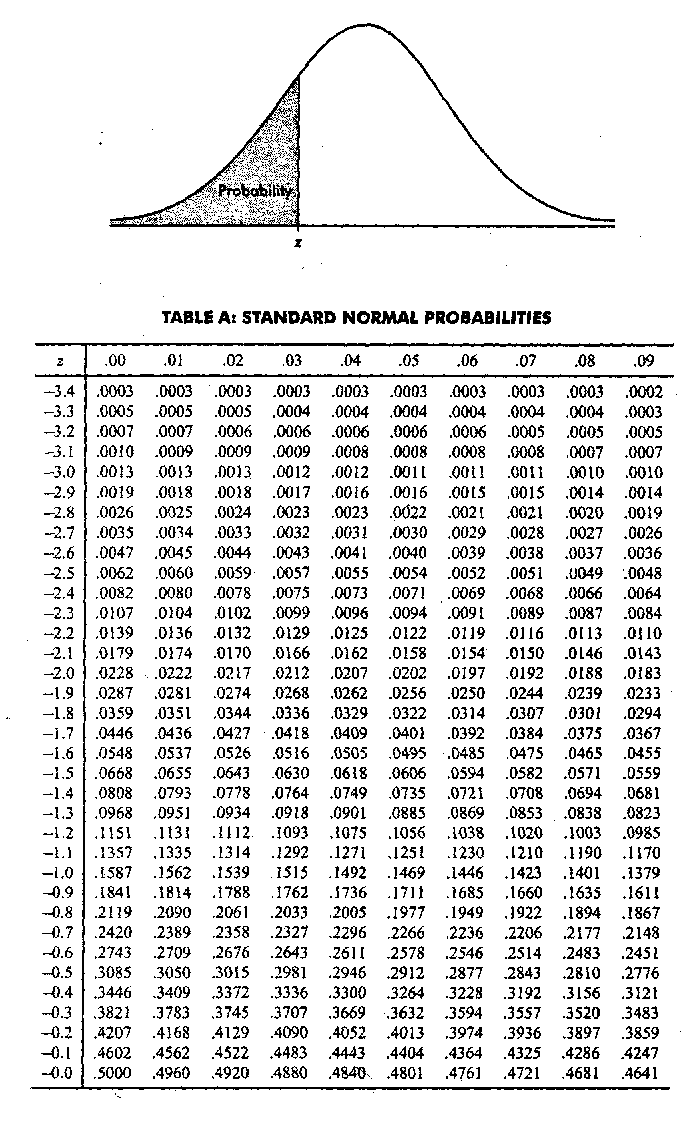
\includegraphics[height=0.9\textheight]{TH_II/z_table}
  \end{figure}
\end{frame}
  
\begin{frame}{Exemplo}
  \begin{example}
    Um neurologista está testando o efeito de uma droga no tempo de
    resposta de um certo estímulo neurológico. Para isto, ele injeta
    uma dose da droga em \alert{100} ratos, cria os estímulos
    neurológicos e observa o tempo de resposta em cada animal. O
    neurologista sabe que o tempo de resposta médio de ratos que não
    receberam a droga é de \alert{1.2 segundos}. O tempo de resposta
    médio dos ratos injetados foi de \alert{1.05 segundos}, com desvio
    padrão amostral de \alert{0.5 segundos}. Você acha que a droga tem
    efeito no tempo de resposta do estímulo?
  \end{example}
Fonte: Khan Academy
\end{frame}

\begin{frame}{Exemplo}
  \begin{example}
    \begin{itemize}
    \item Dados: $\mu = 1.2, \bar{x} = 1.05, s = 0.5, n=100$
    \item $H_0: \mu = 1.2, H_1: \mu < 1.2$ (teste unicaudal à esquerda)
    \item $n$ é grande ($n > 30$), então usamos $\sigma \approx s$ , e
      fazemos o teste Z:
    \item $Z = \frac{1.05 - 1.2}{\frac{0.5}{\sqrt{100}}} = -3$
    \item Consultando a tabela Z, observamos que este Z-escore
      corresponde à probabilidade $p=0.0013$
    \item Como $p < 0.05$, concluímos que há evidência para rejeitar
      $H_0$.
    \end{itemize}
  \end{example}
\end{frame}

\begin{frame}{Tabela Z}
  \begin{figure}
    \centering
      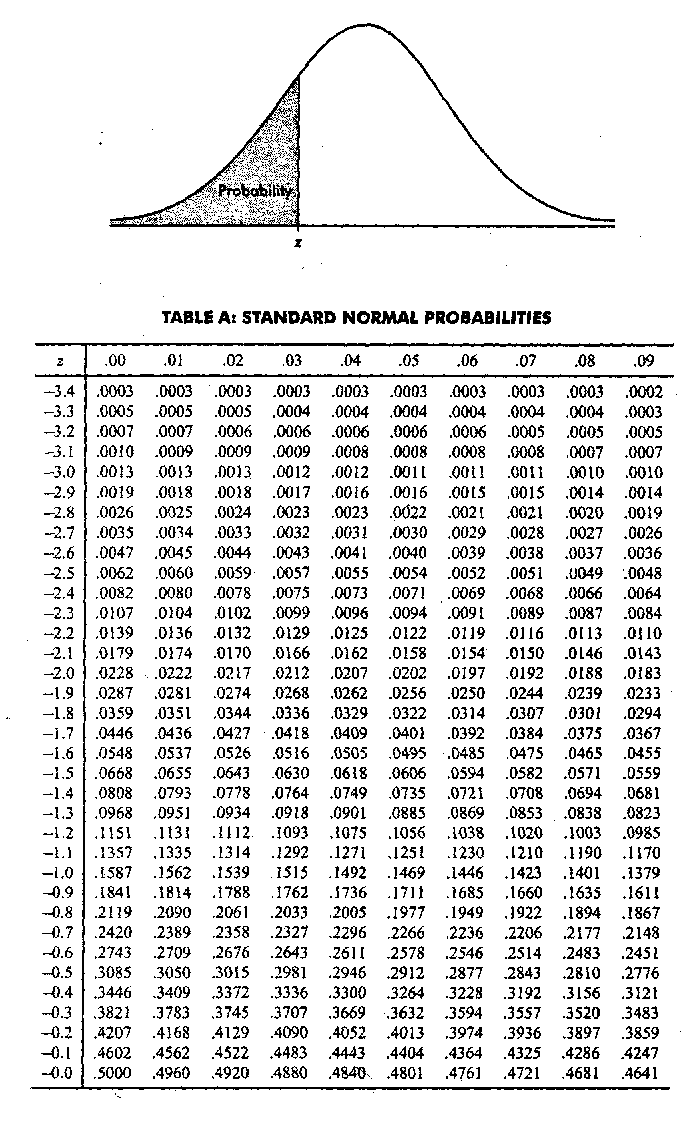
\includegraphics[height=0.9\textheight]{TH_II/z_table}
  \end{figure}
\end{frame}

\begin{frame}{O p-valor}
  Cuidado! O p-valor \alert{não é}:
  \begin{itemize}
  \item a probabilidade de que a hipótese nula seja verdadeira
  \item a probabilidade de que a diferença observada seja devido ao
    acaso
  \end{itemize}
  \begin{block}{}
    Estes são erros comuns de interpretação. 

    O p-valor assume que (1) a hipótese é verdadeira, e (2) que a
    única causa da diferença é devida ao acaso, portanto não pode ser
    usado para concluir suas próprias premissas.
  \end{block}
  \begin{block}{}
    ``The concept of a p value is not simple and any statements
    associated with it must be considered cautiously.''

    Dorey, F. 2010 Clin Orthop Relat Res.
  \end{block}
\end{frame}

\subsection{Resumo}

\begin{frame}{Resumo}
\begin{block}{Interpretação do p-valor}
  \begin{itemize}
  \item Um valor pequeno para o p-valor (tipicamente $p \le 0.05$)
    representa forte evidência para rejeitar a hipótese nula, então
    deve-se rejeitá-la.
  \item Um valor alto para o p-valor (tipicamente $p \ge 0.05$)
    representa pouca evidência contra a hipótese nula, então não se
    deve rejeitá-la
  \item Um valor próximo do ponto de corte ($0.05$) é considerado
    marginal, portanto ``qualquer decisão pode ser tomada''. Sempre
    apresente seu p-valor para que o leitor possa tirar suas próprias
    conclusões.
  \end{itemize}
\end{block}
Fonte: Rumsey, D. (Statistics for Dummies, 2nd ed.)
\end{frame}

\section{Testes com duas amostras}

\begin{frame}{Testes com duas amostras}
  \begin{itemize}
  \item Frequentemente precisamos dividir os dados em dois grupos e
    comparar as médias.
  \item Isto pode ser usado para se estudar o efeito de um tratamento
    em relação a um grupo controle
  \item ou mesmo para se comparar dois tratamentos diferentes.    
  \end{itemize}
\end{frame}

\begin{frame}{Testes com duas amostras}
  \begin{itemize}
  \item Para testar a hipótese de que duas médias $\mu_X$ e $\mu_Y$
    são diferentes, consideramos a diferença $\mu_X - \mu_Y$
  \item Raciocínio: se as médias forem aproximadamente iguais, a
    diferença será aproximadamente zero
  \item Procedemos com o teste de hipótese adequado para a situação
  \end{itemize}
\end{frame}

\begin{frame}{Testes com duas amostras}
Lembre-se que para uma amostra usamos a seguinte estatística de teste:

\begin{displaymath}
  z = \frac{\bar{x} - \mu}{\frac{\sigma}{\sqrt{n}}}
\end{displaymath}

Para duas amostras, é razoável usarmos as estatísticas tanto do grupo
1 quanto do grupo 2.
\end{frame}

\begin{frame}{Testes com duas amostras}
Estatística de teste:

\begin{displaymath}
  z = \frac{ (\bar{x_1} - \bar{x_2}) - (\mu_1 - \mu_2)
  }{\sigma_{(\bar{x_1} - \bar{x_2})}}
\end{displaymath}

onde 

\begin{displaymath}
  \sigma_{(\bar{x_1} - \bar{x_2})} = \sqrt{\frac{\sigma_1^2}{n_1} + \frac{\sigma^2_2}{n_2}}
\end{displaymath}

Mas usaremos uma versão simplificada\ldots
\end{frame}

\begin{frame}{Testes com duas amostras}
  Assumindo que $H_0$ é verdadeira, temos que $\mu_1=\mu_2 \Rightarrow
  \mu_1-\mu_2 = 0$, portanto a estatística de teste que usaremos será:

\begin{displaymath}
  z = \frac{ (\bar{x_1} - \bar{x_2}) }{\sqrt{\frac{\sigma_1^2}{n_1} + \frac{\sigma^2_2}{n_2}}}
\end{displaymath}

\end{frame}

\begin{frame}{Exemplo}
  \begin{example}
    Queremos avaliar a eficiência de uma nova dieta reduzida em
    gordura no tratamento de obesidade. Selecionamos aleatoriamente
    100 pessoas obesas para o grupo 1, que receberão a dieta com pouca
    gordura. Selecionamos outras 100 pessoas obesas para o grupo 2 que
    receberão a mesma quantidade de comida, com proporção normal de
    gordura. Após 4 meses, a perda de peso média no grupo 1 foi de
    9.31 lbs (s=4.67) e no grupo 2 foi de 7.40 lbs (s=4.04). Você acha
    que essa nova dieta é eficaz na perda de peso?
  \end{example}
  Fonte: Khan Academy
\end{frame}

\begin{frame}{Exemplo}
  \begin{example}
    \begin{itemize}
    \item Dados: $\bar{x_1}=9.31, s_1=4.67, \bar{x_2}=7.40, s_2 = 4.04$
    \item $H_0: \mu_1 = \mu_2 \Rightarrow \mu_1 - \mu_2 = 0 \Rightarrow \mu_{(x_1 - x_2)} = 0$
    \item $H_1: \mu_1 - \mu_2 > 0$ (teste unicaudal à direita)
    \item $\bar{x_1}-\bar{x_2}=1.91$
    \item $\sqrt{\frac{\sigma_1^2}{n_1} + \frac{\sigma^2_2}{n_2}} =
      \sqrt{\frac{4.67^2}{100} + \frac{4.04^2}{100}} \approx \alert{0.617}$
    \item Estatística de teste
      \begin{displaymath}
        \alert{z} = \frac{\bar{x_1}-\bar{x_2}}{\sqrt{\frac{\sigma_1^2}{n_1} +
            \frac{\sigma^2_2}{n_2}}} = \frac{1.91}{0.617} \approx \alert{3.09}
      \end{displaymath}
    \end{itemize}
  \end{example}
\end{frame}

\begin{frame}{Tabela Z}
  \begin{figure}
    \centering
      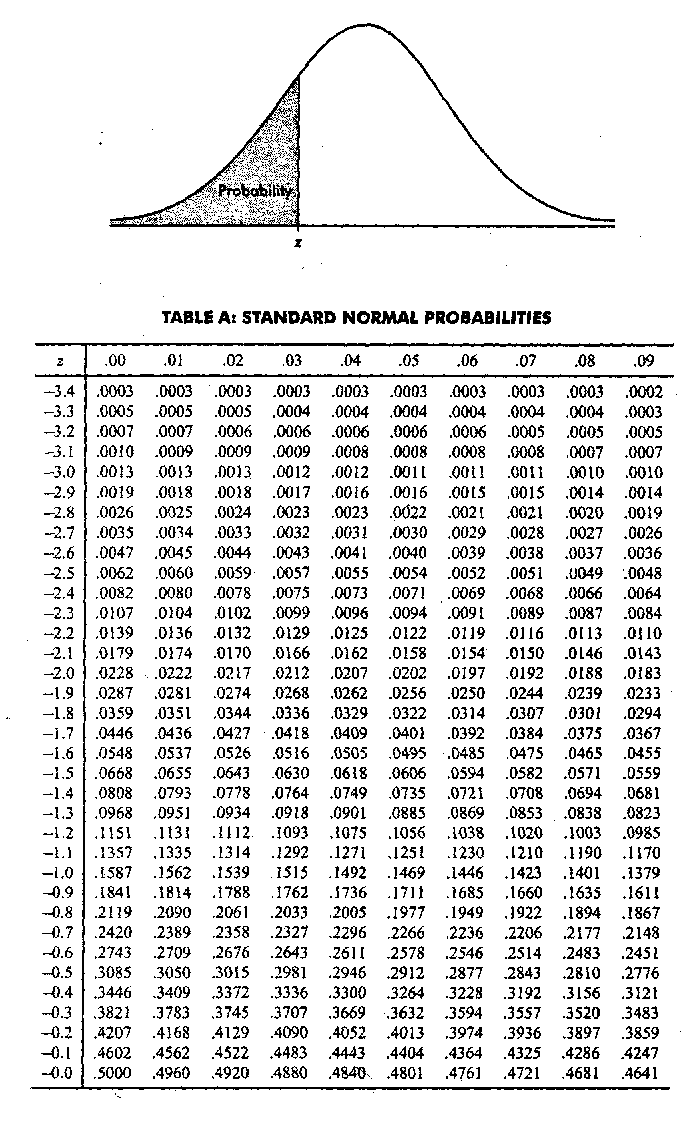
\includegraphics[height=0.9\textheight]{TH_II/z_table}
  \end{figure}
\end{frame}

\begin{frame}{Exemplo}
  \begin{example}
    \begin{itemize}
    \item Encontramos a estatística de teste $z=3.09$
    \item Consultando a tabela Z, a probabilidade correspondente é
      \alert{$p=0.001$}
    \item Como $p<0.05$, concluímos que há evidências para rejeitar $H_0$
    \item Assim, há evidências de que a nova dieta resulta em perda de
      peso
    \end{itemize}
  \end{example}
\end{frame}

% \begin{frame}{Estatísticas de teste para duas amostras}
%   Duas amostras grandes e independentes (teste Z):
%   \begin{displaymath}
%     z = \frac{ (\bar{x_1} - \bar{x_2}) - (\mu_1 - \mu_2)
%     }{\sigma_{(\bar{x_1} - \bar{x_2})}}
%   \end{displaymath}

%   Duas amostras pequenas e independentes (teste t):
%   \begin{displaymath}
%     t = \frac{ (\bar{x_1} - \bar{x_2}) - (\mu_1 - \mu_2)
%     }{\sigma_{(\bar{x_1} - \bar{x_2})}}
%   \end{displaymath}

% % Duas proporções:
% % \begin{displaymath}
% %   z = \frac{(\hat{p_1} - \hat{p_2}) - (p_1-p_2) }{\}
% % \end{displaymath}

% % Duas amostras dependentes (ou emparelhadas):
% % \begin{displaymath}
% % t = \frac{\bar{d} - \mu_d}{\frac{s_d}{\sqrt{n}}}
% % \end{displaymath}
% \end{frame}

\end{document}

